\documentclass[aspectratio=169]{beamer}

\mode<presentation>
{
  \usetheme{default}
  \usecolortheme{default}
  \usefonttheme{default}
  \setbeamertemplate{navigation symbols}{}
  \setbeamertemplate{caption}[numbered]
  \setbeamertemplate{footline}[frame number]  % or "page number"
  \setbeamercolor{frametitle}{fg=white}
  \setbeamercolor{footline}{fg=black}
} 

\usepackage[english]{babel}
\usepackage[utf8x]{inputenc}
\usepackage{tikz}
\usepackage{courier}
\usepackage{array}
\usepackage{bold-extra}
\usepackage{minted}
\usepackage[thicklines]{cancel}

\xdefinecolor{dianablue}{rgb}{0.18,0.24,0.31}
\xdefinecolor{darkblue}{rgb}{0.1,0.1,0.7}
\xdefinecolor{darkgreen}{rgb}{0,0.5,0}
\xdefinecolor{darkgrey}{rgb}{0.35,0.35,0.35}
\xdefinecolor{darkorange}{rgb}{0.8,0.5,0}
\xdefinecolor{darkred}{rgb}{0.7,0,0}
\definecolor{darkgreen}{rgb}{0,0.6,0}
\definecolor{mauve}{rgb}{0.58,0,0.82}

\title[2018-08-02-maynooth-big-data-software]{Big Data Software in Particle Physics}
\author{Jim Pivarski}
\institute{Princeton University -- DIANA-HEP}
\date{August 2, 2018}

\begin{document}

\logo{\pgfputat{\pgfxy(0.11, 7.4)}{\pgfbox[right,base]{\tikz{\filldraw[fill=dianablue, draw=none] (0 cm, 0 cm) rectangle (50 cm, 1 cm);}\mbox{\hspace{-8 cm}
\includegraphics[height=1 cm]{princeton-logo-long.png}
\includegraphics[height=1 cm]{diana-hep-logo-long.png}}}}}

\begin{frame}
  \titlepage
\end{frame}

\logo{\pgfputat{\pgfxy(0.11, 7.4)}{\pgfbox[right,base]{\tikz{\filldraw[fill=dianablue, draw=none] (0 cm, 0 cm) rectangle (50 cm, 1 cm);}\mbox{\hspace{-8 cm}
\includegraphics[height=1 cm]{princeton-logo.png}
\includegraphics[height=1 cm]{diana-hep-logo.png}}}}}

% Uncomment these lines for an automatically generated outline.
%\begin{frame}{Outline}
%  \tableofcontents
%\end{frame}

% START START START START START START START START START START START START START

\begin{frame}{What software should you use in your analysis?}
\large
\vspace{0.75 cm}
\begin{columns}
\column{0.53\linewidth}
Sometimes viewed as a vacuous question, like ``What color is your hammer?''

\vspace{0.75 cm}
\uncover<2->{Anything to get the job done!}
\column{0.4\linewidth}
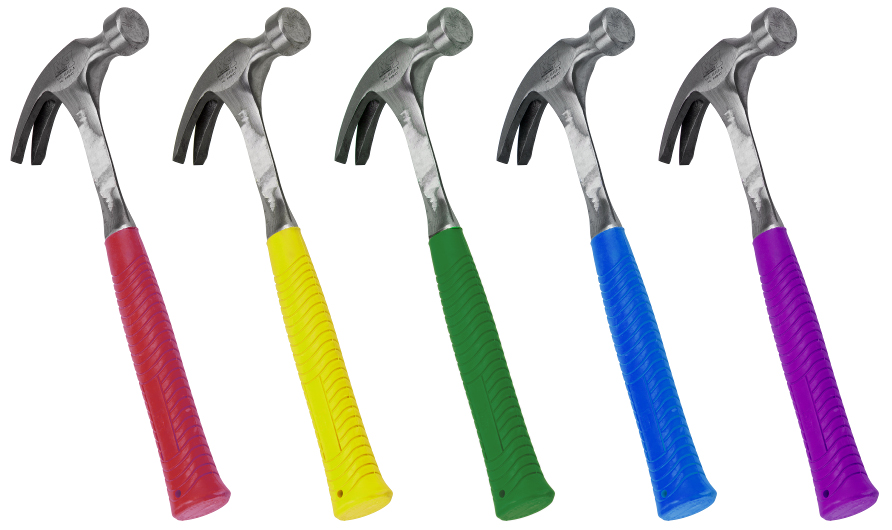
\includegraphics[width=\linewidth]{hammer.jpg}
\end{columns}

\vspace{0.75 cm}
\uncover<3->{\Large \textcolor{darkblue}{But there are real differences and sometimes it matters:}}

\large
\vspace{0.1 cm}
\begin{itemize}\setlength{\itemsep}{0.2 cm}
\item<4-> Tool for the wrong problem \hfill (hammer vs.\ screwdriver)
\item<5-> Ease of use/productivity of data analyst \hfill (ergonomics of handle)
\item<6-> Computational performance \hfill (sledge hammer weight)
\end{itemize}
\end{frame}

\begin{frame}{}
\vspace{1 cm}
\begin{center}
\huge \textcolor{darkblue}{Why this matters now:}

\vspace{0.5 cm}
\large we're not the only ones analyzing big datasets anymore: ``web scale analytics''
\end{center}
\end{frame}

\begin{frame}{\only<1>{We measure globally distributed data in hundreds of PB}\only<2>{But for ``web scale'' companies, 100 PB = 1 truck}}
\vspace{0.35 cm}
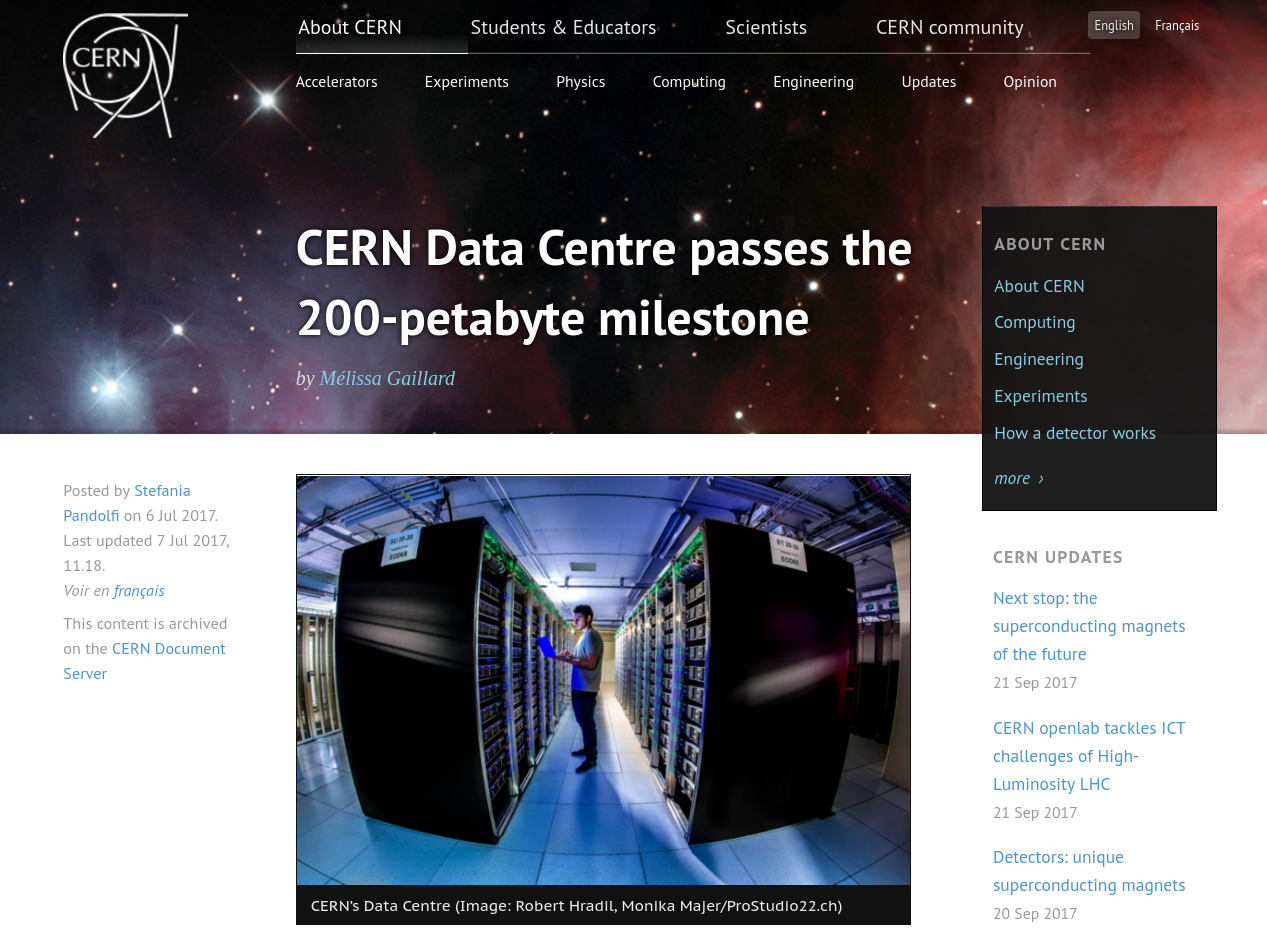
\includegraphics[width=0.73\linewidth]{cern-200pb.png}

\vspace{-4.8 cm}
\uncover<2->{\mbox{ } \hfill 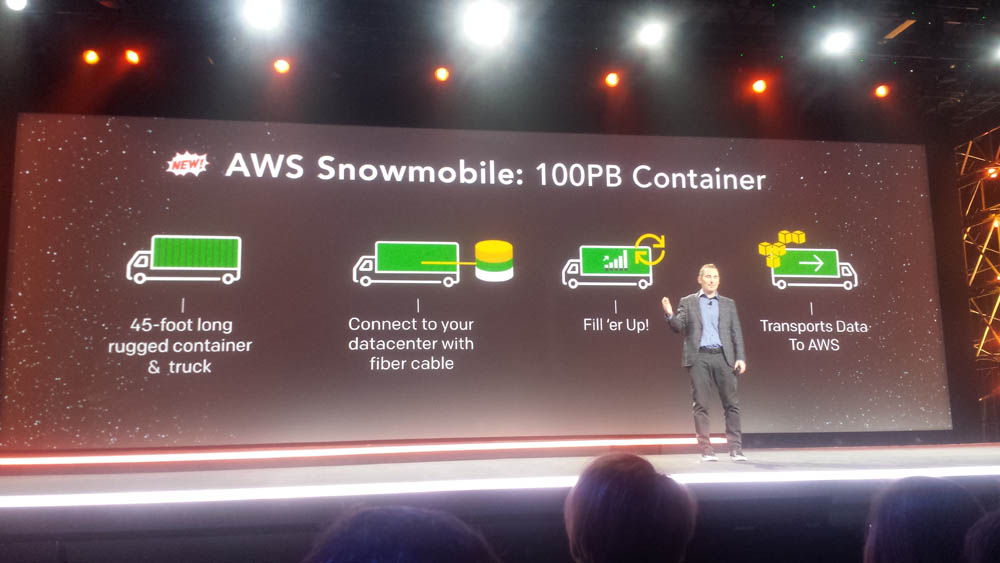
\includegraphics[width=0.7\linewidth]{aws-snowmobile.jpg}\hspace{-1 cm}}
\end{frame}

\begin{frame}{Recently developed, but many eyes on the code\ldots}
\vspace{0.5 cm}
\begin{center}
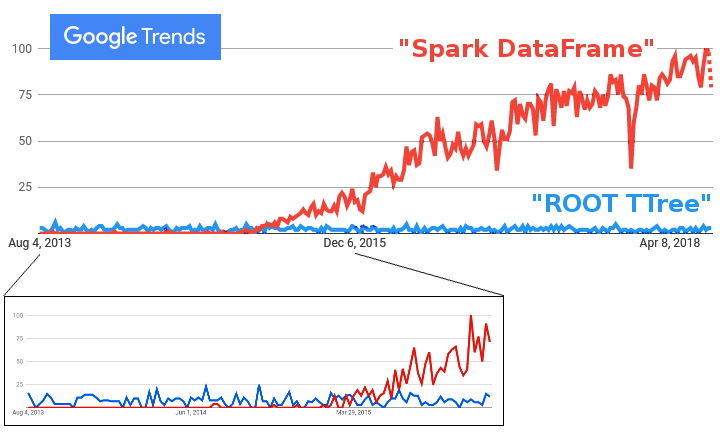
\includegraphics[width=0.8\linewidth]{root-spark-google-trends.png}
\end{center}
\end{frame}

\begin{frame}{Their ecosystem developed largely independently of ours}
\vspace{0.17 cm}
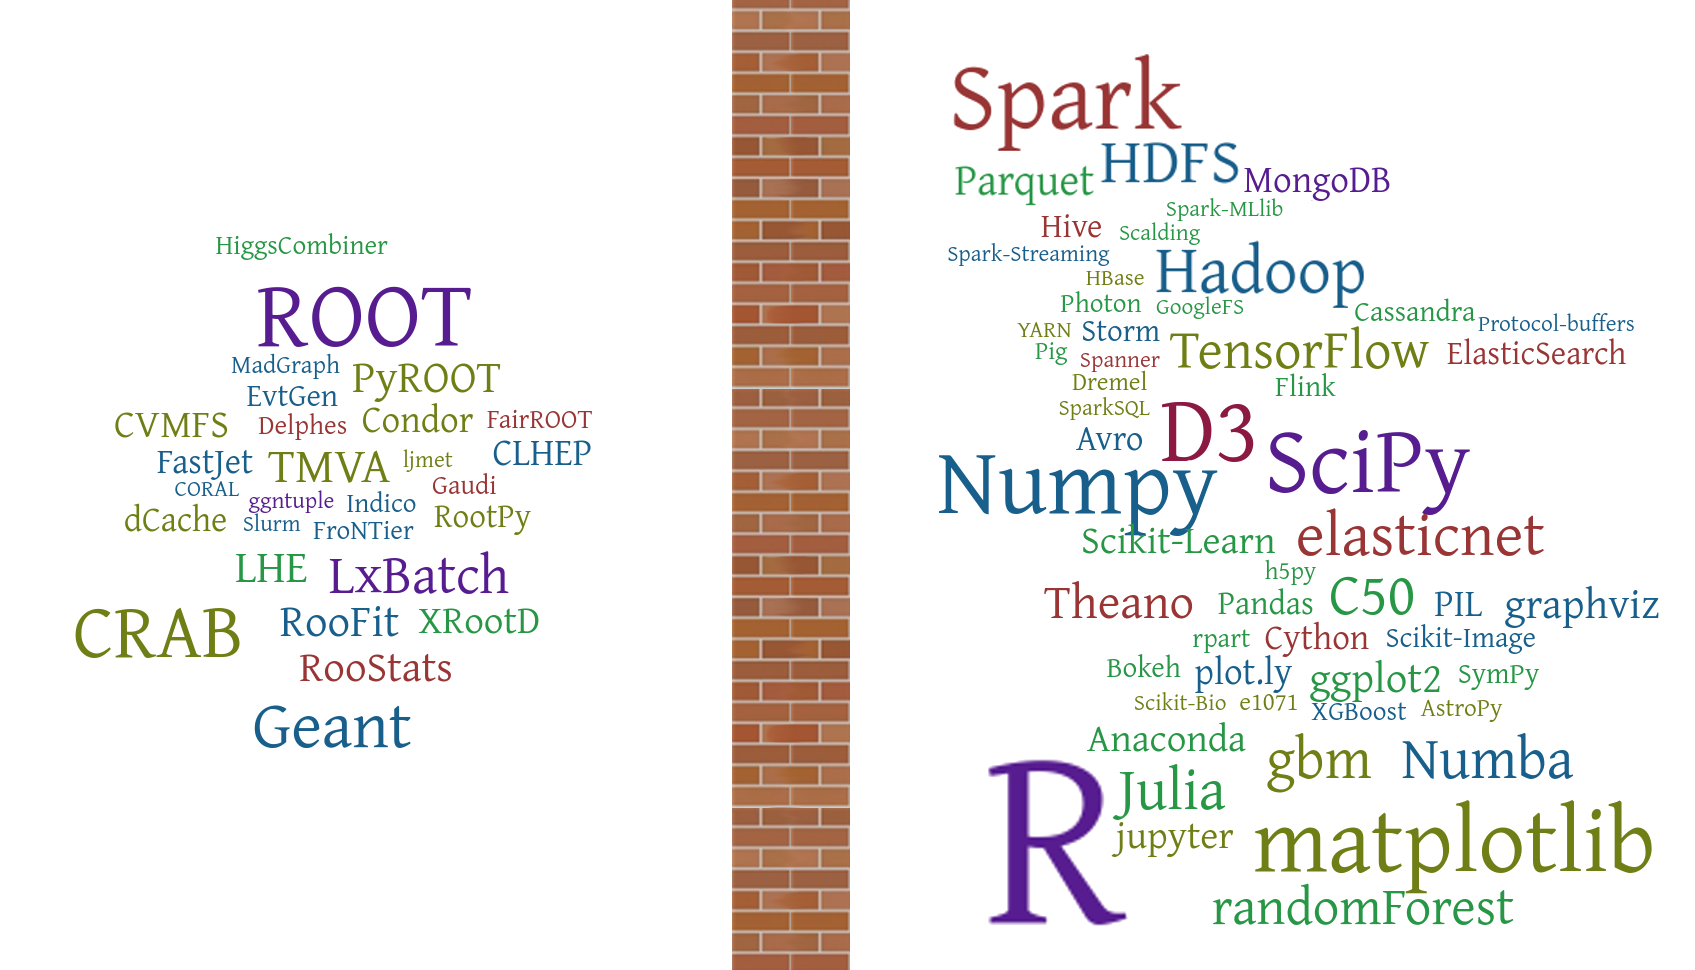
\includegraphics[width=\linewidth]{separation-2.png}
\end{frame}

\begin{frame}{Ideally, we should use the strengths of both}
\vspace{0.5 cm}
\large
\begin{columns}[t]
\column{0.5\linewidth}
\textcolor{darkblue}{\underline{What we can find off the shelf}}

\vspace{0.1 cm}
\begin{itemize}\setlength{\itemsep}{0.1 cm}
\item distributed processing, scale-out
\item C++/Python interoperability
\item special functions, matrix math
\item fitting/minimization, integration, differentiation, interpolation
\item symbolic algebra
\item advanced statistics
\item machine learning
\item graphics, advanced plotting
\item graphical interfaces, user workflows
\end{itemize}

\column{0.5\linewidth}
\textcolor{darkblue}{\underline{What we still must develop in-house}}

\vspace{0.1 cm}
\begin{itemize}\setlength{\itemsep}{0.1 cm}
\item reading/writing ROOT files
\item collaboration frameworks, triggers, event reconstruction
\item advanced histogramming and fitting
\item efficient variable-length lists \\ (our kind of non-relational data)
\item domain-specific functions
\end{itemize}
\end{columns}
\end{frame}

\begin{frame}[fragile]{Distributed processing: Spark}
\vspace{0.5 cm}
\begin{columns}[b]
\column{0.59\linewidth}
\textcolor{darkblue}{\Large \underline{Functional programming, managed data:}}

\large
\vspace{0.25 cm}
\begin{itemize}
\item Big, distributed dataset is a local variable

\scriptsize
\begin{minted}{python}
lookup = spark.textFile("lookup.txt").map(int)
table  = spark.cassandraTable("T").filter("col > 0")
both   = table.join(lookup).where("n == N")
cached = both.map("x**2 + y**2").cache()
hist   = cached.reduce(histogram)
cached.saveAsTextFile("tmp.txt")
\end{minted}
\end{itemize}

\column{0.35\linewidth}
\tiny

\textcolor{blue}{\url{http://www.cs.sfu.ca/CourseCentral/732/ggbaker/content/spark.html}}

\vspace{0.2 cm}
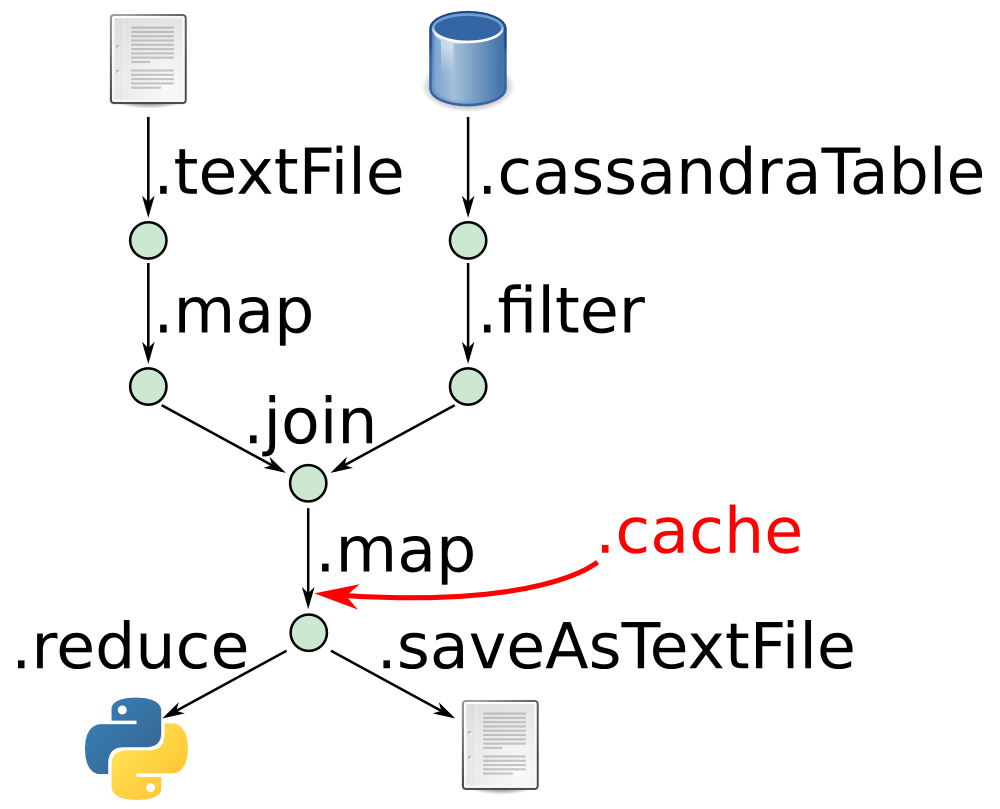
\includegraphics[width=\linewidth]{spark-dag.png}
\end{columns}

\large
\begin{itemize}
\item Reduction or saving triggers a distributed job
\item Spark manages files, dependencies, retry-on-failure
\item Distributed dataset may be in RAM (fast), disk (big), or both (spill-over)
\end{itemize}
\end{frame}

\begin{frame}[fragile]{Accessing particle physics data in Spark}
\large
\vspace{0.5 cm}
\begin{description}
\item[Spark-ROOT:] presents a large set of ROOT files as a Spark DataFrame

\small
\begin{minted}{python}
mydata = (spark.read.format("org.dianahep.sparkroot")
                    .option("tree", "Events")
                    .load("many-files/*.root"))
\end{minted}

\normalsize
\textcolor{blue}{\url{https://github.com/diana-hep/spark-root}}
\large

\vspace{0.5 cm}
\item[XRootD-HDFS:] presents an XRootD service (e.g.\ EOS) as HDFS for Spark

\small
\begin{minted}{python}
...load("hdfs://eos.cern.ch/many-files/*.root")
\end{minted}

\normalsize
\textcolor{blue}{\url{https://github.com/opensciencegrid/xrootd-hdfs}}
\end{description}

\vspace{0.5 cm}
\uncover<2->{\fbox{\begin{minipage}{0.95\linewidth} ROOT's new RDataFrame adds a Spark-like interface to local ROOT files; potential for driving Spark from ROOT in the future. \end{minipage}}}
\end{frame}

\begin{frame}{Awkwardness of Spark}
\Large
\vspace{0.5 cm}
\begin{columns}
\column{1.05\linewidth}
\begin{center}
\textcolor{darkorange}{\bf Spark runs on Java Virtual Machines (ubiquitous in business).}

\vspace{1 cm}
\uncover<2->{\textcolor{darkgreen}{Hard to interface C++ (especially ROOT) with Java; \\ PySpark performance is limited by its Java-Python tunnel.}}

\vspace{1 cm}
\uncover<3->{\textcolor{mauve}{Python itself is much more open to interoperability with C++, \\ has similar distributed computing projects: Dask, Joblib, Parsl\ldots}}
\end{center}
\end{columns}
\end{frame}

\begin{frame}{Data analysis ecosystem has grown around Python}
\vspace{0.25 cm}
\begin{columns}[b]
\column{0.75\linewidth}
\only<1>{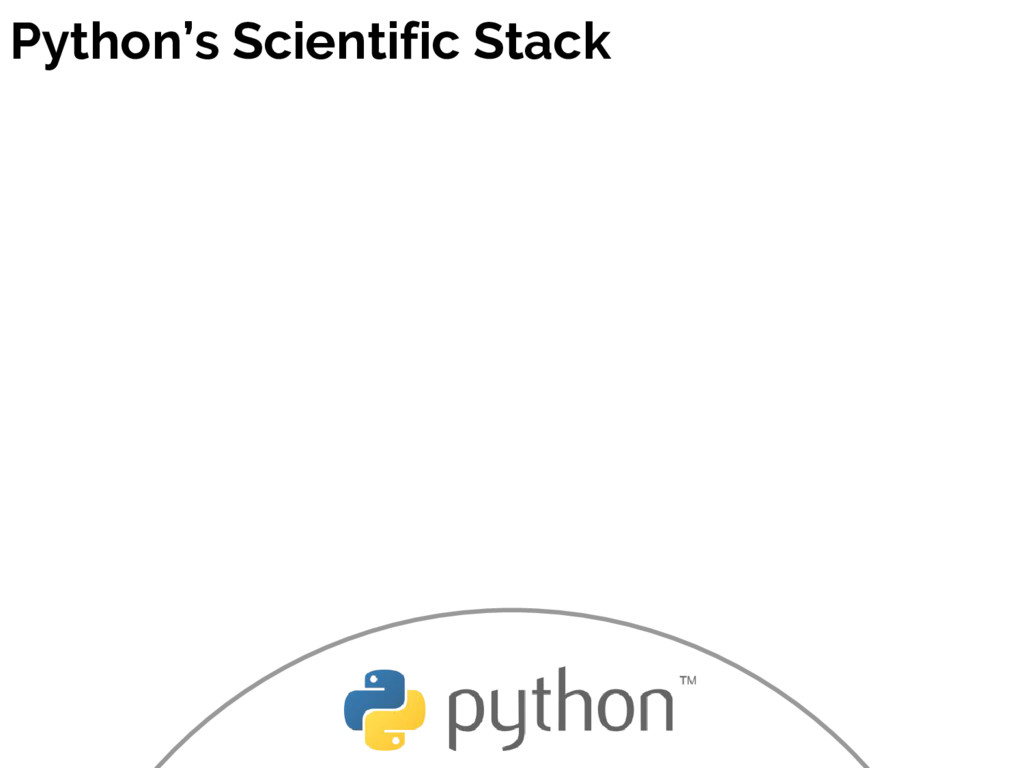
\includegraphics[height=7.8 cm]{shells-1.png}}
\only<2>{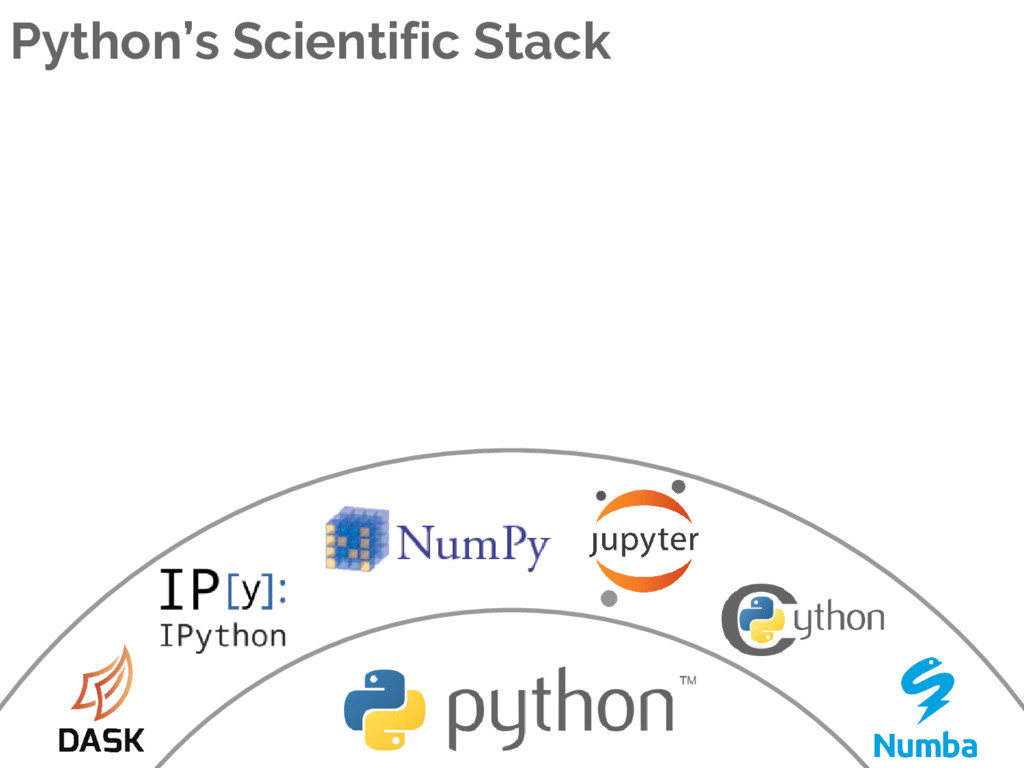
\includegraphics[height=7.8 cm]{shells-2.png}}
\only<3>{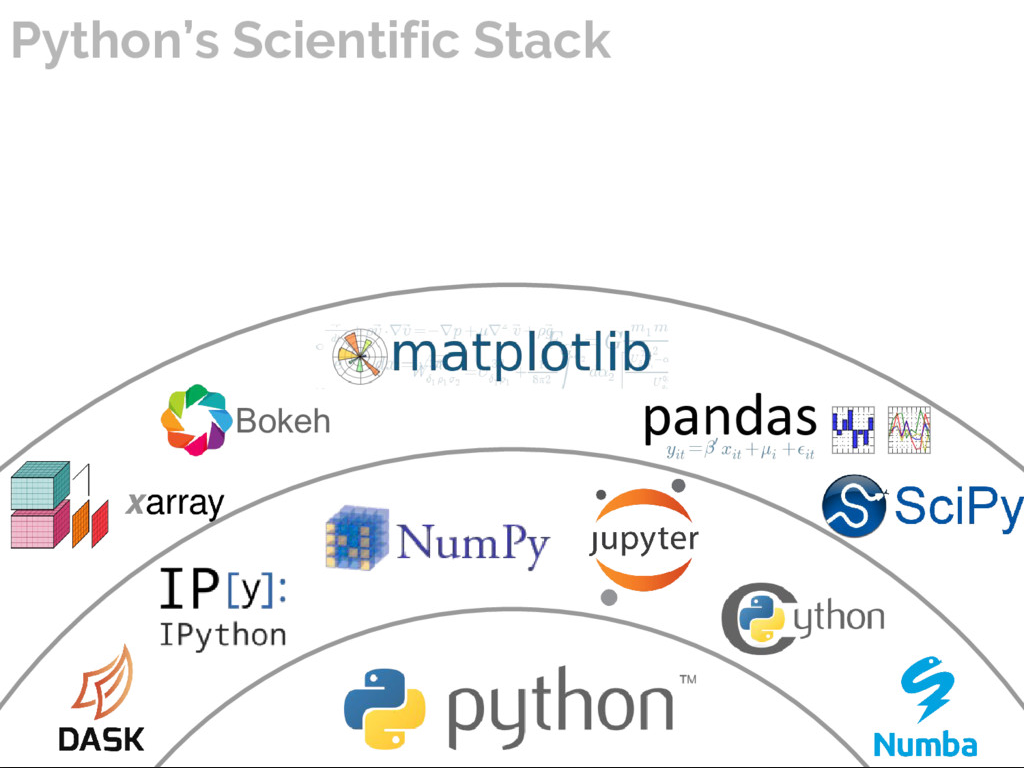
\includegraphics[height=7.8 cm]{shells-3.png}}
\only<4>{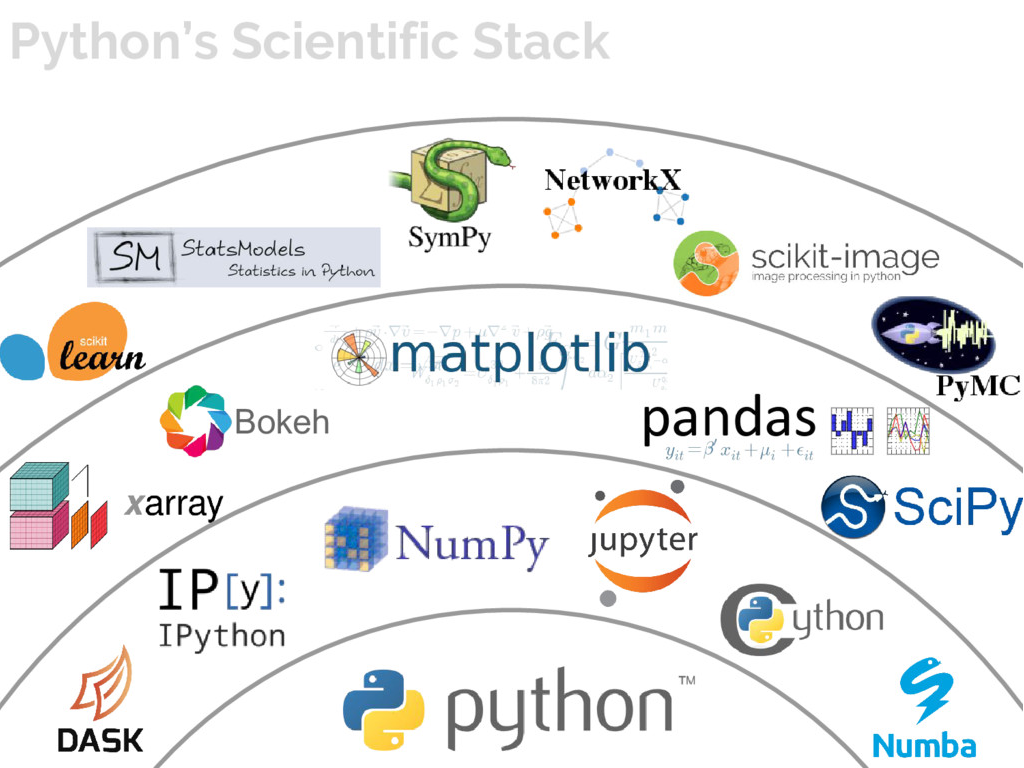
\includegraphics[height=7.8 cm]{shells-4.png}}
\only<5>{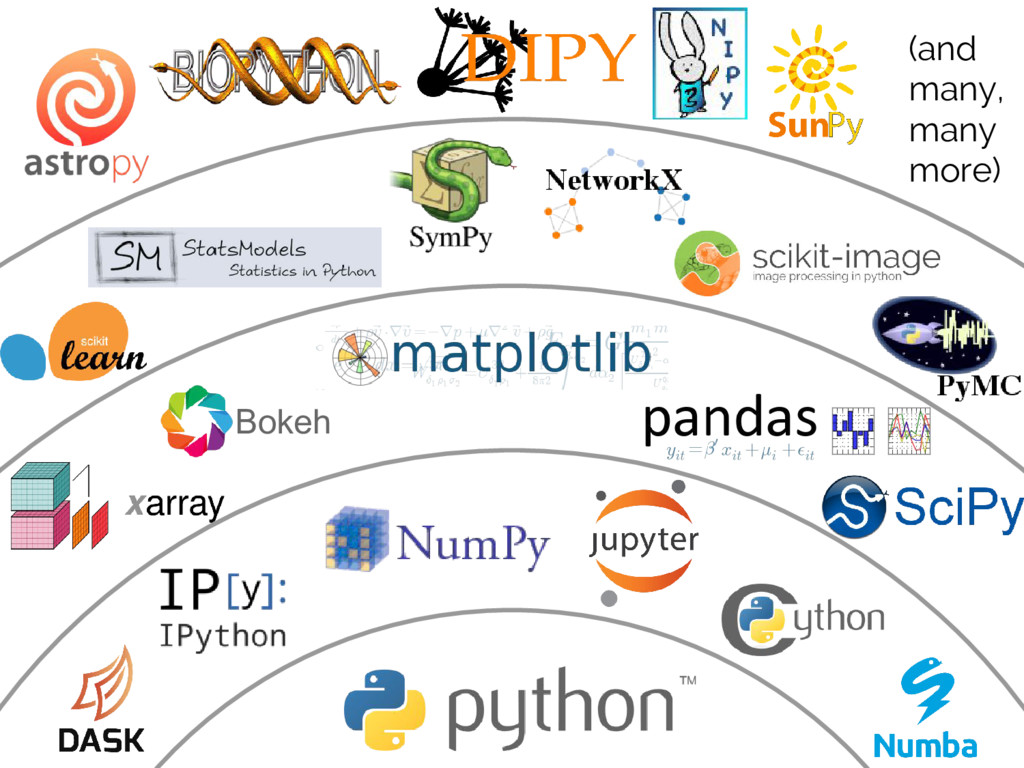
\includegraphics[height=7.8 cm]{shells-5.png}}

\column{0.25\linewidth}

\includegraphics[width=\linewidth]{unreasonable-effectiveness.png}
\vspace{5.3 cm}
\end{columns}
\end{frame}

\begin{frame}{Particularly machine learning}
\vspace{0.5 cm}
\mbox{ } 
\includegraphics[height=0.8 cm]{sklearn-logo.png}
\hfill 
\includegraphics[height=0.8 cm]{pytorch-logo.png}
\hfill 
\includegraphics[height=0.8 cm]{keras-logo.png}
\hfill 
\includegraphics[height=1 cm]{tensorflow-logo.png}
\hfill 
\includegraphics[height=0.8 cm]{caffe2-logo.png}
\hfill 
\includegraphics[height=0.8 cm]{gluon-logo.png} \mbox{ }

\vspace{0.15 cm}
\mbox{ } 
\includegraphics[height=0.8 cm]{chainer-logo.png}
\hfill 
\includegraphics[height=0.8 cm]{cntk-logo.png}
\hfill 
\includegraphics[height=0.8 cm]{lasagne-logo.png}
\hfill 
\includegraphics[height=0.8 cm]{onnx-logo.png}
\hfill 
\includegraphics[height=0.8 cm]{cesium-logo.png}
\hfill 
\includegraphics[height=0.8 cm]{xgboost-logo.png} \mbox{ }

\vspace{1.5 cm}
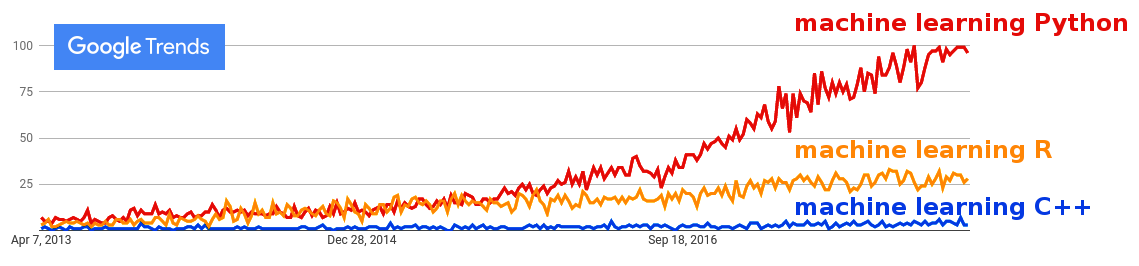
\includegraphics[width=\linewidth]{python-r-cpp-googletrends-machinelearning.png}
\end{frame}

\begin{frame}{In some fields, adoption is astronomical\ldots}
\vspace{0.25 cm}
\begin{center}
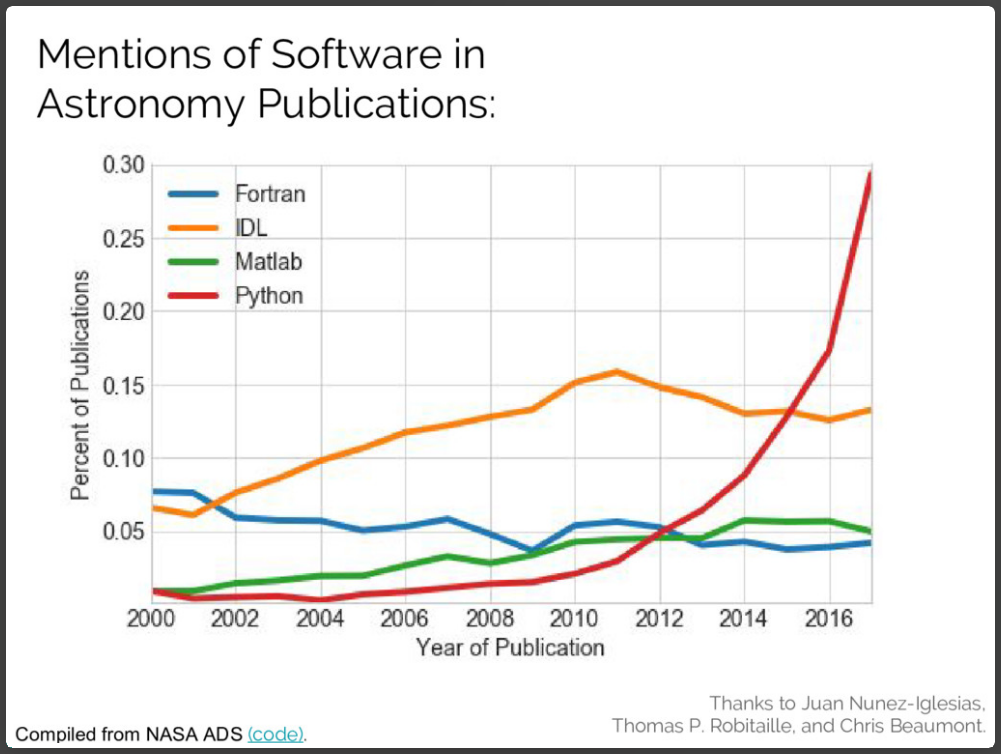
\includegraphics[width=0.7\linewidth]{mentions-of-programming-languages.png}
\end{center}
\end{frame}

\begin{frame}{Accessing ROOT data in Python}
\large
\vspace{0.5 cm}
\begin{description}\setlength{\itemsep}{0.5 cm}
\item[PyROOT:] general solution but slow if called in a loop over events; new ROOT features like {\normalsize\tt TTree::AsMatrix()} fill Numpy arrays directly, but only for primitive types.

\item[root\_numpy:]<2-> good solution for many years, except slow for nested data (e.g.~{\normalsize\tt std::vector<float>}) and compiles against a version of ROOT: changing ROOT version causes binary incompatibility.

\item[uproot:]<3-> reimplementation of ROOT I/O in Python+Numpy, skipping a step that is unnecessary for filling arrays:

\vspace{0.5 cm}
\mbox{ } \hfill bytes of ROOT file $\to$ \only<3>{C++ objects}\only<4>{\xcancel{C++ objects}} $\to$ Numpy arrays \hfill \mbox{ }
\end{description}
\end{frame}


\end{document}
